\section{Laser Shock Peening}

Laser Shock Peening (LSP) treatment induces residual stresses beneath the treated surface of metallic materials. The residual stresses are produced by a high magnitude shock wave induced by a high-energy laser pulse. The advantage of LSP is that the laser pulse can be adjusted and controlled in real time. A computer-controlled system can measure the energy per pulse and record it for each LSP process on the component [Mannava 1998].

\subsection{Laser Shock Peening Process}
The configuration of an LSP process on a metallic component is shown in Figure \ref{fig:lspconfiguration}. An intense pulsed laser shock beam is fired onto a metal surface for a brief time (10-100 ns). The heated zone is vaporized and transformed to plasma by ionization due to high temperatures (over 10 000 °C). The plasma is under high pressure, which propagates through the material via shock waves. Two modes of LSP exist – the direct ablation mode and the confined ablation mode. The direct ablation mode refers to the interaction of plasma with metal without coating and confinement. Plasma pressure of tenths of a GPa is achieved using direct ablation mode. Higher pressures of 5-10 GPa can be obtained using the confined mode. In the confined mode, the metal surface is usually coated with an opaque material such as black paint or aluminium foil and confined by a material transparent to the laser radiation such as distilled water or borosilicate glass. A stronger pressure pulse results in a higher magnitude of compressive residual stress to a deeper depth.

\begin{figure}[h]
    \centering
    
\includegraphics[width=0.6\linewidth]{img/lsp_configuration.jpg}
    \caption{Schematic configuration of laser shock peening}
    \label{fig:lspconfiguration}
\end{figure}

\subsection{Laser Shock Peening Strategy}
During the peening process, a pattern is created made of individual laser pulses. Generally, multiple sequences of the pattern that are gradually shifted across the sample are used to create a layer, as seen in Figure No \ref{fig:lspstrategy}. The pattern shifting ensures a more homogeneous residual stress distribution. This peening strategy's disadvantage is that the protective coating needs to be replaced in between sequences.

\begin{figure}[h]
    \centering
    
\includegraphics[width=0.6\linewidth]{img/lsp_strategy.jpg}
    \caption{Laser shock peening strategy - one layer consisting of four sequences}
    \label{fig:lspstrategy}
\end{figure}

\section{LSP station and laser source at HiLASE Centre}

The LSP station uses the Bivoj laser system, located on the ground floor of the HiLASE Centre. A Laser Beam Distribution System (LBDS) transports the beam to
experimental laboratories on the 1\textsuperscript{st} floor. The Bivoj laser
system is a Diode Pumped Solid State Laser (DPSSL) based on
Yb-doped gain media with a laser wavelength of 1030 nm
capable of delivering energy pulses up to 8 J at a 10 Hz
repetition rate. The beam shape at the output of the Bivoj laser is a
square flat-top pulse. An overview of the BIVOJ laser system is shown in Figure \ref{fig:bivoj}. The two main sections of the Bivoj laser are
the front-end and the 10 J amplifier.

\begin{figure}[h]
    \centering
    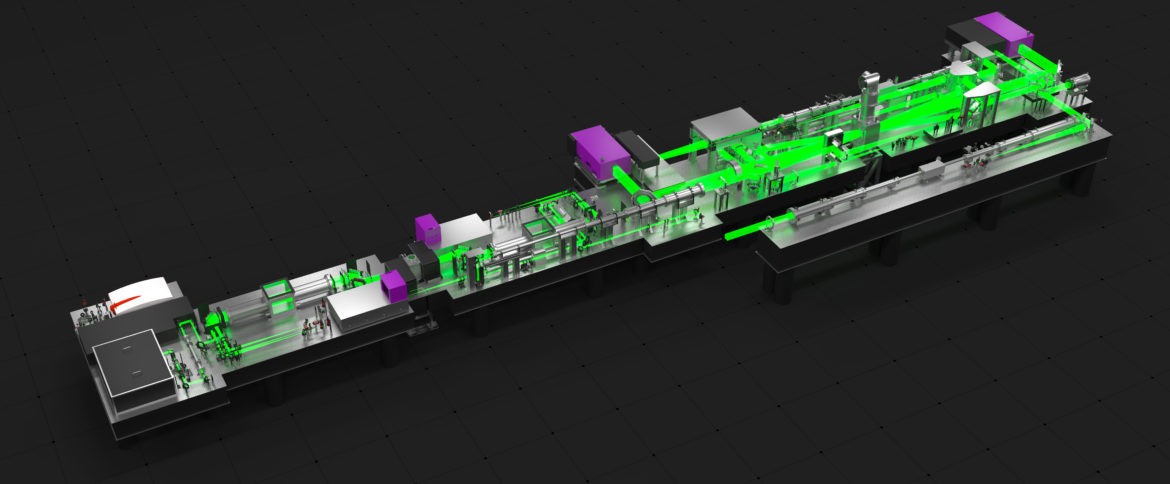
\includegraphics[width=1.0\linewidth]{img/bivoj.jpg}
    \caption{LASER SYSTEM "BIVOJ": Diode-pumped solid-state (DPSSL) laser DiPOLE 100}
    \label{fig:bivoj}
\end{figure}

\subsection{Bivoj front-end}

The front end starts with a fibre-based section, consisting
of a fibre oscillator, fibre amplifier and temporal pulse shaper
with 125 ps resolution. The output of the fibre front-end is fed
to the first booster amplifier, which is regenerative and
increases the energy to 3 mJ and reduces the repetition rate to 10
Hz. The second booster amplifier works in a multi-pass regime
and increases the pulse energy to approximately 30 mJ.
The repetition rate can be chosen between 1 Hz and 10 Hz. The
beam shape at the front-end output is 8x8 mm2 square flat top.

\subsection{Bivoj 10 J amplifier}

The 10 J amplifier is the first-stage main amplifier based on
cryogenically cooled multi-slab technology. The principal
component of the amplifier is the amplifier head, where the
gain media are stored and cooled by gaseous helium to 
the temperature of about 150 K. The laser beam from the front-end
is enlarged to 21*21 mm\textsuperscript{2} and sent to the 10 J amplifier, where
increases its pulse energy from approximately 30 mJ to
approximately 6 J at 10 Hz.

\subsection{LSP station layout}

The layout of the LSP station is as shown in Figure \ref{fig:lsplayout}. The laser
beam enters the LSP station through the LSP output node and
continues to the optical table, where it is redirected and
focused on the target. The target itself is mounted on the
robotic arm. The laser beam position is fixed, so the robotic
arm needs to be moved to direct the laser.

\begin{figure}[h]
    \centering
    
\includegraphics[width=0.6\linewidth]{img/lsp_layout.jpg}
    \caption{Schematic layout of LSP station}
    \label{fig:lsplayout}
\end{figure}
